\chapter{Generative Adversarial Networks}
\graphicspath{{figs/2de/}}

This exploration delves into the realm of generative models, specifically focusing on Generative Adversarial Networks (GANs) and their conditional variants. GANs have emerged as a groundbreaking concept in unsupervised learning that revolutionized image generation and manipulation. The objective is not only to comprehend the technical mechanisms of GANs but also to recognize their profound impact on image generation, editing, and completion. This exploration also highlights how these models are reshaping our approach to generative tasks within the field of machine learning in a broader context.

\section{Generative Adversarial Networks}

This section presents Generative Adversarial Networks (GANs), a deep learning framework that employs two neural networks, a generator, and a discriminator, in a competitive setup. It offers fundamental insights into how these networks collaborate to produce synthetic data instances that closely resemble real data. The focus is on understanding the architecture, the training procedure, and the core principles, laying the foundation for their various applications in areas such as image generation, style transfer, and beyond.

\subsection{General principles}

\begin{align}
    \min_{G} & \max_{D} \mathbb{E}_{x^* \sim \mathcal{D}\text{ata}} \left[ \log D(x^*) \right] + \mathbb{E}_{z \sim P(z)} \left[ \log (1 - D(G(z))) \right] \label{eq:minimax}        \\
             & \max_{G} \mathbb{E}_{z \sim P(z)} \left[ \log D(G(z)) \right] \label{eq:G_maximization}                                                                                \\
             & \max_{D} \mathbb{E}_{x^* \sim \mathcal{D}\text{ata}} \left[ \log D(x^*) \right] + \mathbb{E}_{z \sim P(z)} \left[ \log (1 - D(G(z))) \right] \label{eq:D_maximization}
\end{align}

\paragraph*{1. Interpret the equations \ref{eq:G_maximization} and \ref{eq:D_maximization}. What would happen if we only used one of the two?}

\Cref{eq:G_maximization} describes the goal of the generator $G$ in a GAN. The generator aims to produce images $\tilde{x} = G(z)$ that are indistinguishable from real images by the discriminator. The objective function for the generator maximizes the probability of the discriminator incorrectly classifying these generated images as real. In other words, the generator is trained to "fool" the discriminator. A higher value of $D(G(z))$ implies that the discriminator is more likely to mistake the generated image for a real one, indicating a better performance of the generator.

\Cref{eq:D_maximization} describes the goal of the discriminator $D$ in a GAN. The discriminator's role is to distinguish between real images $x^*$ from the dataset and fake images $\tilde{x}$ produced by the generator. The objective function for the discriminator is to maximize the sum of two terms: the probability of correctly identifying real images as real, and the probability of correctly identifying generated images as fake. The first term $\left(\mathbb{E}_{x^* \sim \mathcal{D}\text{ata}} \left[ \log D(x^*) \right]\right)$ encourages the discriminator to correctly classify real images as real, while the second term $\left(\mathbb{E}_{z \sim P(z)} \left[ \log (1 - D(G(z))) \right]\right)$ pushes it to correctly identify the synthetic images as fake.

If we only used the generator's objective function (\ref{eq:G_maximization}) without the discriminator, the generator would not have a reliable way to measure how good its generated images are. It would lack the feedback mechanism that the discriminator provides, leading to poor-quality image generation. Conversely, if we only used the discriminator's objective function (\ref{eq:D_maximization}) without the generator, the discriminator would only learn to distinguish real images from a static set of fake images. It would not adapt to improving fake images, making it less effective over time as it would not be challenged by increasingly realistic fake images. A GAN relies entirely on the interplay between the generator and discriminator: the generator improves by trying to fool the discriminator, while the discriminator becomes better at distinguishing real from fake images, leading to a dynamic and effective learning process.

\paragraph*{2. Ideally, what should the generator $G$ transform the distribution $P(z)$ to?}

Ideally, the generator $ G $ in a GAN should transform the input noise distribution $ P(z) $ into a distribution that closely resembles the real data distribution $ P(X) $.

In a GAN, $ z $ is a vector sampled from a predefined noise distribution $ P(z) $, which is typically a uniform or normal distribution. The role of the generator $ G $ is to map this noise vector $ z $ into a data point $ \tilde{x} = G(z) $ that appears to have been drawn from the distribution of real data $ P(X) $. The success of the generator is measured by how indistinguishable its output $ \tilde{x} $ is from real data points when evaluated by the discriminator.

The end goal is for the distribution of the generated data $ P_G(X) $ (where $ X $ is generated by $ G(z) $ for $ z \sim P(z) $) to be as close as possible to the real data distribution $ P(X) $. When this happens, the discriminator should find it increasingly difficult to tell apart real data from the generated data, ideally reaching a point where it performs no better than random guessing, resulting in equilibrium, i.e. $\forall x, \, D(x) = 1/2$. This signifies that the generator has effectively learned to produce data that mimics the real data distribution. 

\paragraph*{3. Remark that the equation \ref{eq:G_maximization} is not directly derived from the equation \ref{eq:minimax}. This is justified by the authors to obtain more stable training and avoid the saturation of gradients. What should the ''true'' equation be here?}

In the concept of a GAN, the generator's goal is ideally defined as minimizing the likelihood that the discriminator correctly identifies its outputs as fake. Mathematically, this gives us the following ''true'' equation:

\[
    \min_{G} \mathbb{E}_{z \sim P(z)} \left[ \log (1 - D(G(z))) \right]
\]

This objective aims for the generator to produce images that the discriminator will classify as fake (i.e., it tries to minimize the probability of the discriminator being correct).

\subsection{Architecture of the networks}

\paragraph*{4. Comment on the training of the GAN with the default settings (progress of the generations, the loss, stability, image diversity, etc.).}

In our GAN training, we observed a notable progression in the quality of generated images as the training advanced. However, the loss values exhibit significant instability, oscillating across epochs, which is a common trait in GAN training, indicating their tendency not to converge in practice. This means that while training over 5 epochs, neither $G$ nor $D$ wins decisively, but $D$ has a tendency to perform better at the game, i.e., it manages to identify the fake images, which in turn encourages $G$ to produce better images. 

While the generator does improve image quality over time, the generated results still appear noticeably synthetic and limited in diversity, primarily resembling digits such as 0, 3, 7, and 8. This observation raises concerns about a potential mode collapse issue, where the generator learns to produce only a subset of possible outputs that are sufficient to deceive the discriminator but lacks overall diversity.

For a detailed reference, please consult the training curves in \Cref{fig:longer_epochs_losses}, where the 5-epoch mark corresponds to 2300 steps, and review the generated images after 5 epochs in \Cref{fig:default}.

\begin{figure}[H]
    \centering
    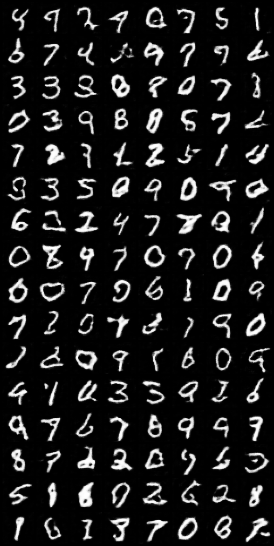
\includegraphics[width=0.2\textwidth]{default.png}
    \label{fig:default}
    \caption{Generated images after 5 epochs, using the default settings.}
\end{figure}

\newpage
\paragraph*{5. Comment on the diverse experiences that you have performed with the suggestions above. In particular, comment on the stability on training, the losses, the diversity of generated images, etc.}

To conduct our experiments, we developed a PyTorch-Ignite framework, which is included alongside this report for reference. This framework played a crucial role in ensuring the reproducibility and traceability of our experiments. It's worth noting that the curves presented in our results represent the number of total iterations, calculated as the number of epochs multiplied by the batch size. Consequently, it's normal to observe peaks in the curves, which indicate the start of a new epoch during training.

\paragraph*{Longer epochs}
In our experiments, we initially extended the training to 30 epochs. In deep learning, it's a common practice that more epochs can contribute to improved stability. Beyond the 10th epoch, we noticed consistent convergence in subsequent epochs. Further analysis of the training curves, depicted in \Cref{fig:longer_epochs_losses}, revealed that the discriminator's output, $D(x)$, approached 1, and the discriminator's output for generated images, $D(G(z))$, approached 0. This essentially means that the discriminator perfectly distinguished real images from fake images, indicating that the discriminator was winning the adversarial game, while the generator was losing, which is not the outcome we are looking for. 

This situation prompted an intriguing observation when observing the generation process during training, as shown in \Cref{fig:longer_epochs}. We observed the evolution of the background in these images. Originally black, it gradually developed a form of noise. This phenomenon can be attributed to the generator's struggle to produce better digits. When it cannot improve the quality of the digits, it starts generating noise as a way to produce something different. If we were to continue training for even longer, we might end up with completely noisy images. 

This observation underscores the delicate balance in GAN training. Increasing the number of epochs can be risky, as it can lead to the discriminator becoming proficient at distinguishing between real and fake images, causing the generator to resort to generating noise to try and deceive the discriminator.

In conclusion, it's important to note that as training progresses, the discriminator may start giving more and more random feedback, and the generator might train on uninformative feedback, resulting in a decrease in the quality of its generated outputs. As a result, convergence in GANs is often a temporary state rather than a stable and permanent condition.

\begin{figure}[!htbp]
    \centering

    \begin{subfigure}{0.2\textwidth}
        \centering
        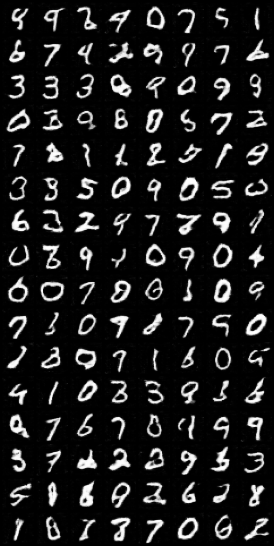
\includegraphics[width=0.95\linewidth]{longer_epochs/fake_sample_epoch_0010.png}
        \caption{}
        \label{subfig:longer_epochs/fake_sample_epoch_0010}
    \end{subfigure}%
    \begin{subfigure}{0.2\textwidth}
        \centering
        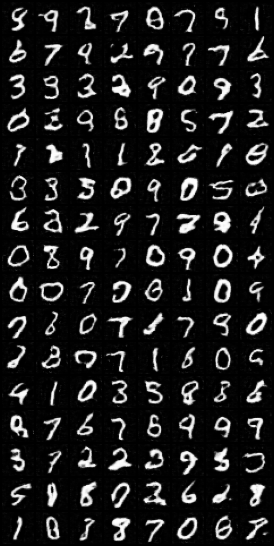
\includegraphics[width=0.95\linewidth]{longer_epochs/fake_sample_epoch_0015.png}
        \caption{}
        \label{subfig:longer_epochs/fake_sample_epoch_0015}
    \end{subfigure}%
    \begin{subfigure}{0.2\textwidth}
        \centering
        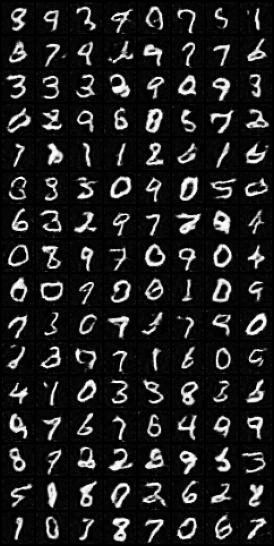
\includegraphics[width=0.95\linewidth]{longer_epochs/fake_sample_epoch_0020.png}
        \caption{}
        \label{subfig:longer_epochs/fake_sample_epoch_0020}
    \end{subfigure}%
    \begin{subfigure}{0.2\textwidth}
        \centering
        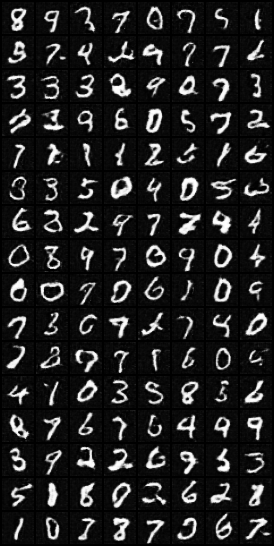
\includegraphics[width=0.95\linewidth]{longer_epochs/fake_sample_epoch_0025.png}
        \caption{}
        \label{subfig:longer_epochs/fake_sample_epoch_0025}
    \end{subfigure}%
    \begin{subfigure}{0.2\textwidth}
        \centering
        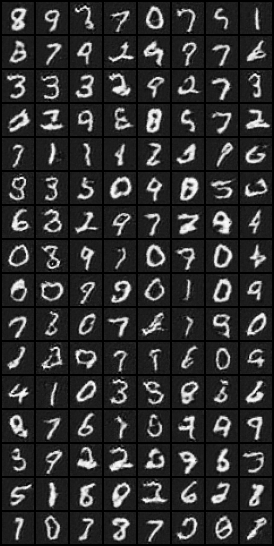
\includegraphics[width=0.95\linewidth]{longer_epochs/fake_sample_epoch_0030.png}
        \caption{}
        \label{subfig:longer_epochs/fake_sample_epoch_0030}
    \end{subfigure}%

    \caption{Generated images during training after (a) 10 epochs, (b) 15 epochs, (c) 20 epochs, (d) 25 epochs and (e) 30 epochs.}
    \label{fig:longer_epochs}
\end{figure}

\begin{figure}[H]
    \centering

    \begin{subfigure}{0.45\textwidth}
        \centering
        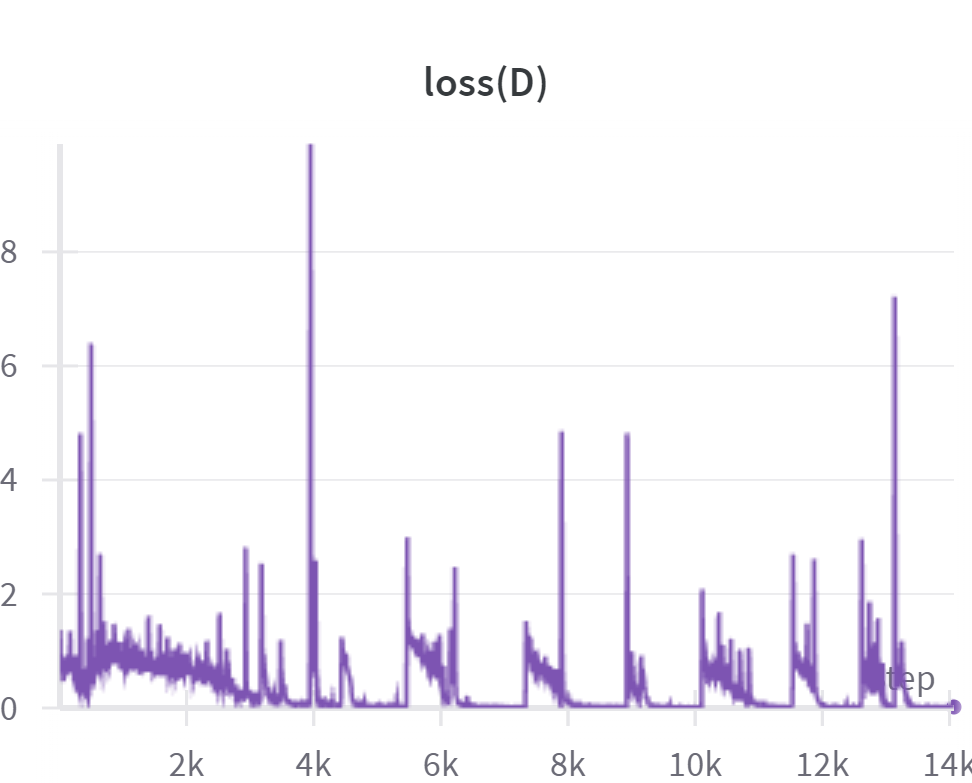
\includegraphics[width=0.95\linewidth]{longer_epochs/lossD.png}
        \caption{}
        \label{subfig:longer_epochs/lossD}
    \end{subfigure}%
    \begin{subfigure}{0.45\textwidth}
        \centering
        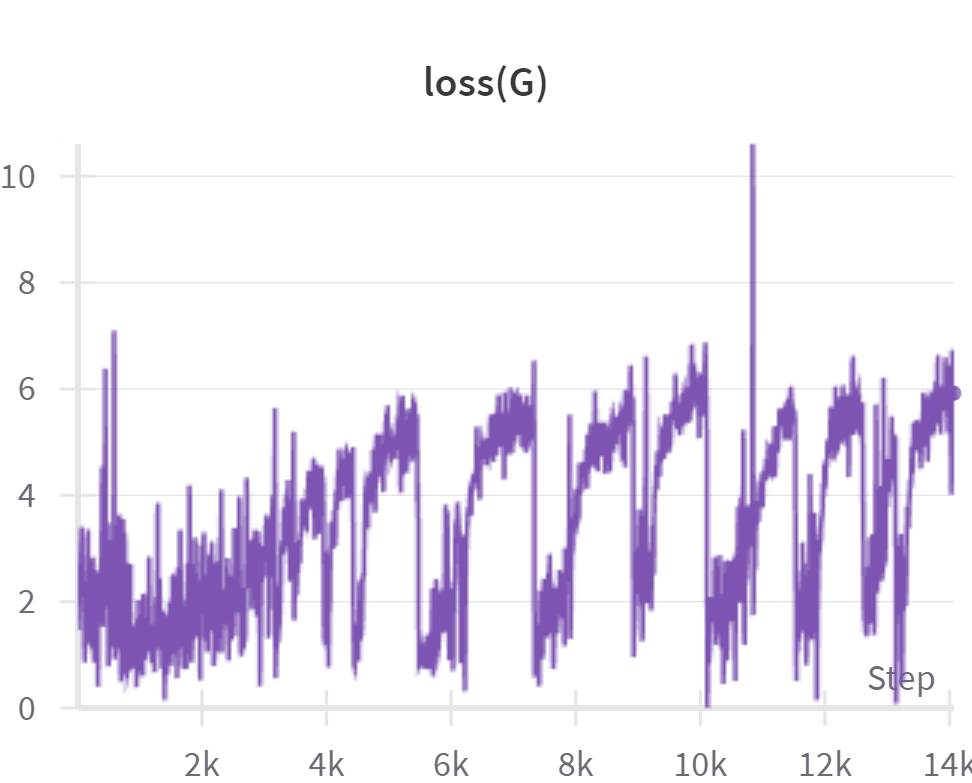
\includegraphics[width=0.95\linewidth]{longer_epochs/lossG.png}
        \caption{}
        \label{subfig:longer_epochs/lossG}
    \end{subfigure}

    \begin{subfigure}{0.45\textwidth}
        \centering
        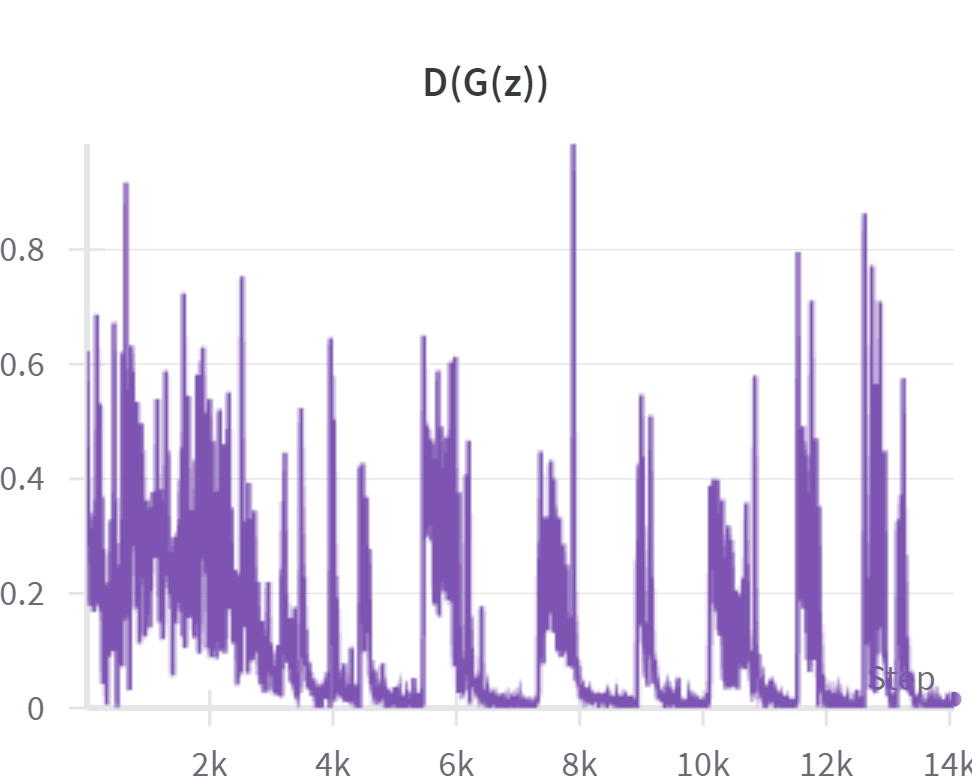
\includegraphics[width=0.95\linewidth]{longer_epochs/D_G_z.png}
        \caption{}
        \label{subfig:longer_epochs/D_G_z}
    \end{subfigure}%
    \begin{subfigure}{0.45\textwidth}
        \centering
        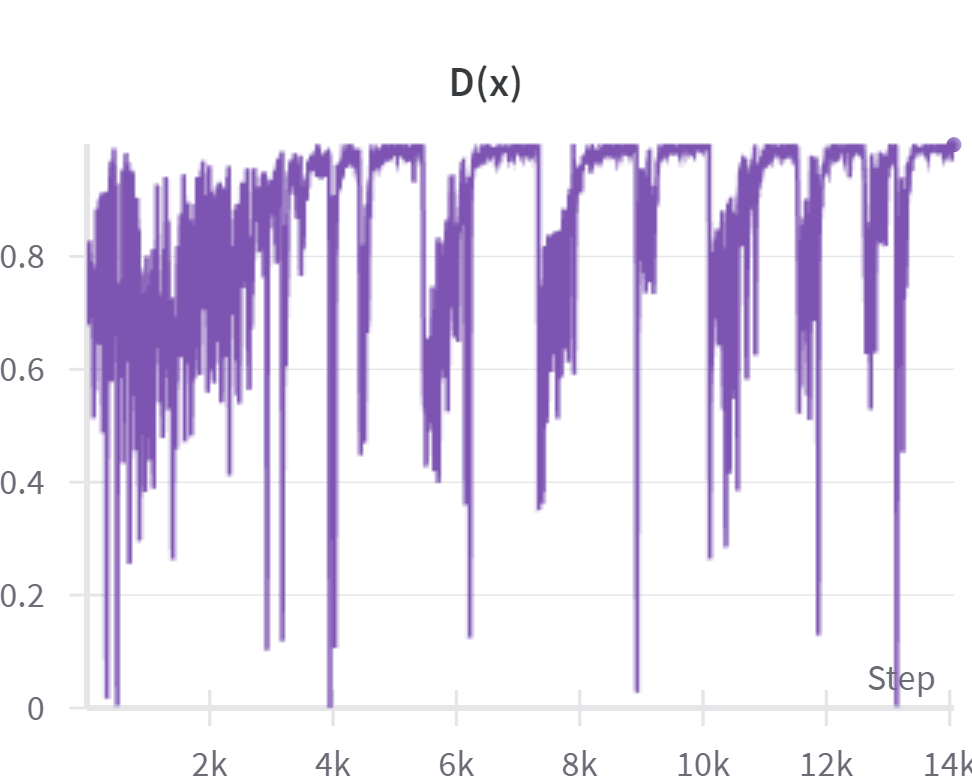
\includegraphics[width=0.95\linewidth]{longer_epochs/D_x.png}
        \caption{}
        \label{subfig:longer_epochs/D_x}
    \end{subfigure}

    \begin{subfigure}{0.45\textwidth}
        \centering
        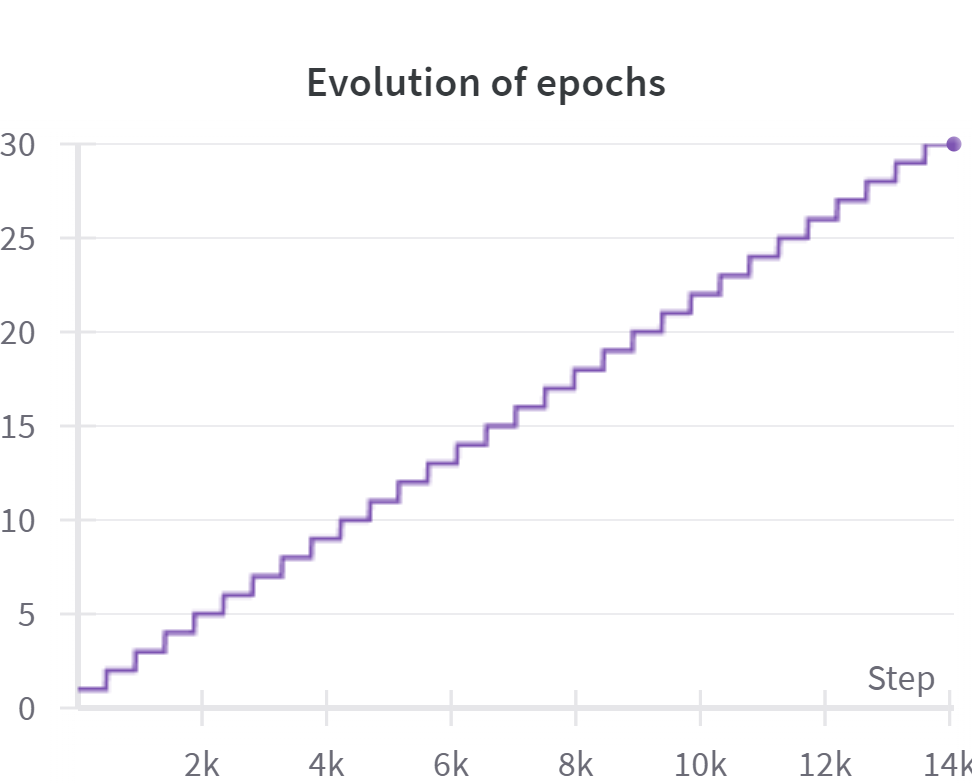
\includegraphics[width=0.95\linewidth]{longer_epochs/epochs.png}
        \caption{}
        \label{subfig:longer_epochs/epochs}
    \end{subfigure}%

    \caption{Training curves: (a) $loss(D)$, (b) $loss(G)$, (c) $D(G(z))$, (d) $D(x)$ and (e) the number of epochs by the number of iterations.}
    \label{fig:longer_epochs_losses}
\end{figure}



\paragraph*{Influence of $n_z$}
We conducted an investigation to explore the impact of varying the size of the noise vector ($n_z$), a parameter that plays a role in determining the diversity and complexity of the generated images. The results of this experiment are presented in \Cref{fig:nz}.

Analyzing only the losses and the discriminator's output values, there doesn't appear to be a significant difference between the various values of $n_z$. This suggests that the impact of $n_z$ on the training process may not be fully reflected in these metrics alone.

However, when we consider the generated images themselves, we observe more significant differences. Decreasing the value of $n_z$ resulted in a reduction in the diversity of the generated outputs but allowed the model to produce good quality images more quickly. On the other hand, increasing the value of $n_z$ enhanced diversity among the generated images but introduced greater complexity to the training process. These observations indicate that the choice of $n_z$ has a more noticeable impact on the visual diversity and complexity of the generated images compared to its effect on training metrics like losses and discriminator outputs.

\begin{figure}[H]
    \centering

    \begin{subfigure}{0.2\textwidth}
        \centering
        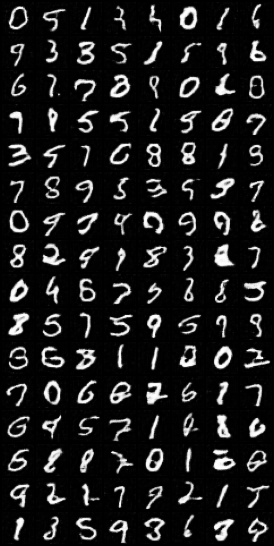
\includegraphics[width=0.95\linewidth]{nz/nz10_fake_sample_epoch_0010.png}
        \caption{}
        \label{subfig:nz10}
    \end{subfigure}%
    \begin{subfigure}{0.2\textwidth}
        \centering
        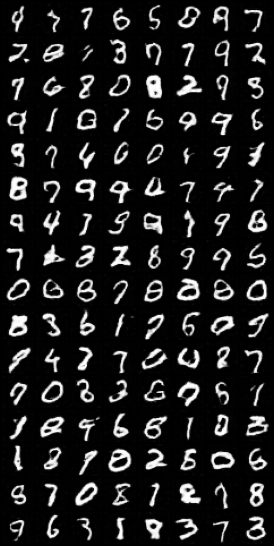
\includegraphics[width=0.95\linewidth]{nz/nz50_fake_sample_epoch_0010.png}
        \caption{}
        \label{subfig:nz50}
    \end{subfigure}%
    \begin{subfigure}{0.2\textwidth}
        \centering
        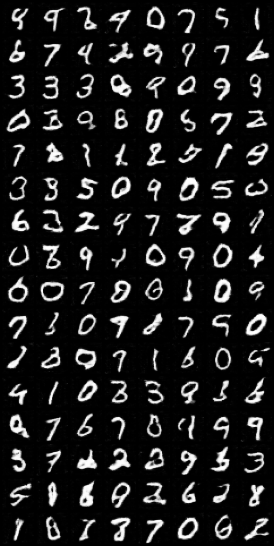
\includegraphics[width=0.95\linewidth]{nz/nz100_fake_sample_epoch_0010.png}
        \caption{}
        \label{subfig:nz100}
    \end{subfigure}%
    \begin{subfigure}{0.2\textwidth}
        \centering
        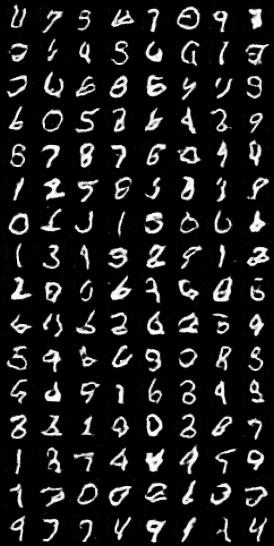
\includegraphics[width=0.95\linewidth]{nz/nz500_fake_sample_epoch_0010.png}
        \caption{}
        \label{subfig:nz500}
    \end{subfigure}%
    \begin{subfigure}{0.2\textwidth}
        \centering
        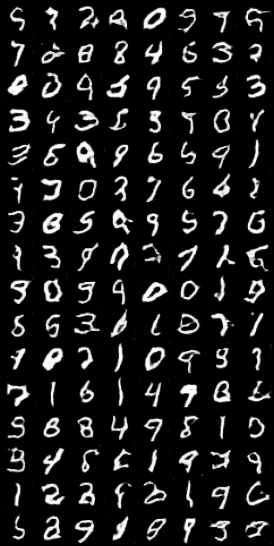
\includegraphics[width=0.95\linewidth]{nz/nz1000_fake_sample_epoch_0010.png}
        \caption{}
        \label{subfig:nz1000}
    \end{subfigure}%
    \caption{Generated images after being trained for 10 epochs with (a) $ n_z = 10 $ (b) $ n_z = 50 $ (c) $ n_z = 100 $ (d) $ n_z = 500 $ and (e) $ n_z = 1000 $.}
    \label{fig:nz}
\end{figure}

\paragraph*{Influence of weight initialization}
Upon switching to PyTorch's default weight initialization, we observed higher error rates throughout the training process. Additionally, the quality of the generated images was less convincing when using the default weight initialization compared to the results obtained with the optimized parameters. This outcome highlights the significant impact of customized weight initialization in GANs, as it affects both the training efficiency and the overall quality of the generated images.

\begin{figure}[H]
    \centering

    \begin{subfigure}{0.2\textwidth}
        \centering
        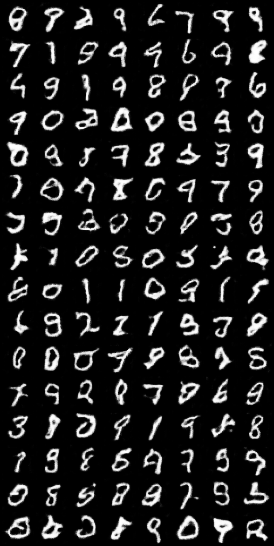
\includegraphics[width=0.95\linewidth]{init/fake_sample_epoch_0005.png}
        \caption{}
        \label{subfig:init/fake_sample_epoch_0005}
    \end{subfigure}%
    \begin{subfigure}{0.2\textwidth}
        \centering
        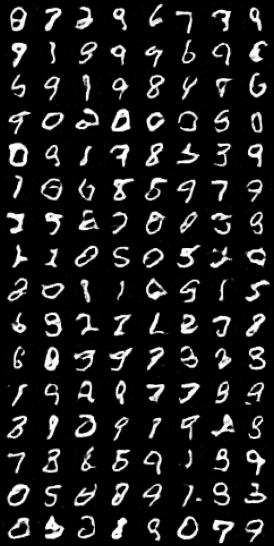
\includegraphics[width=0.95\linewidth]{init/fake_sample_epoch_0010.png}
        \caption{}
        \label{subfig:init/fake_sample_epoch_0010}
    \end{subfigure}%
    \begin{subfigure}{0.2\textwidth}
        \centering
        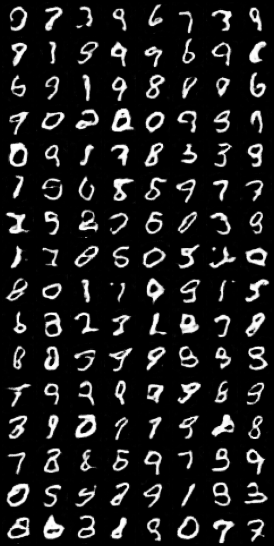
\includegraphics[width=0.95\linewidth]{init/fake_sample_epoch_0015.png}
        \caption{}
        \label{subfig:init/fake_sample_epoch_0015}
    \end{subfigure}%

    \caption{Generated images during training with default PyTorch weight initialization after (a) 5 epochs, (b) 10 epochs and (c) 15 epochs.}
    \label{fig:init}
\end{figure}

% we then changed the weights to use the default ones of pytorch. notably, the gan takes a bit longer to converge 11 epoch and the errors are highers. moreover, the generated images are less convincing that the ones generated using optimized paramers.

\paragraph*{Influence of $ngf$ and $ndf$}

% in searching to generate better images, we modified $ngf$ , as Changing the number of generator or discriminator filters can affect the quality and detail of generated images. it lead in a heavier training time. mopreover, the images generated were much clearer. [comment on the losses and errors with the image i provide]

\paragraph*{Trying CIFAR-10 dataset}

Unfortunately, due to Google Drive limitations, we were unable to perform experiments using CelebA. Instead, we conducted experiments on CIFAR-10, a dataset of more complex images. We trained a GAN over 15 epochs on $32 \times 32$ generated images. It's important to note that the generated images won't match the beauty of those in the dataset due to the reduced resolution. However, this experiment yielded interesting results.

One notable observation is that the generator had difficulty distinguishing the generated images from the real images, as indicated by the training curves in \Cref{fig:cifar10_32_curves}. We have provided the generated images in \Cref{fig:cifar10_32_images}. While at first glance, these images may appear indistinct, they still exhibit characteristics that suggest they were generated from CIFAR-10. This implies that the generator has learned the underlying distribution of the images, even though the generated images themselves may not be visually appealing due to the limited resolution.

\begin{figure}[H]
    \centering

    \begin{subfigure}{0.45\textwidth}
        \centering
        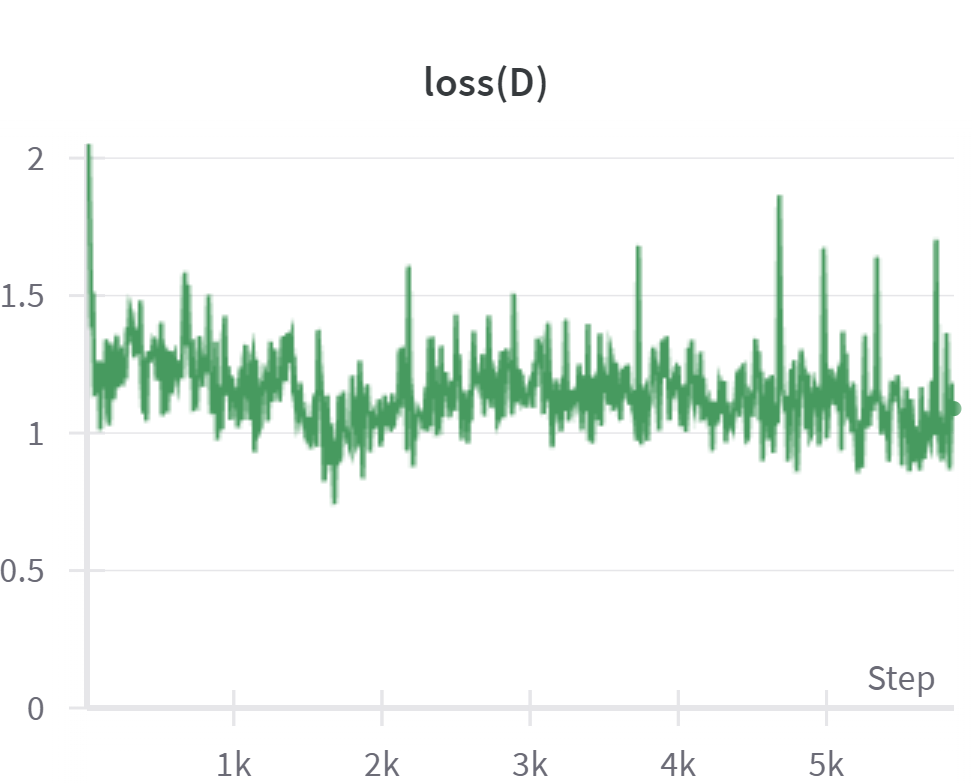
\includegraphics[width=0.95\linewidth]{cifar10/32/lossD.png}
        \caption{}
        \label{subfig:cifar10/32/lossD}
    \end{subfigure}%
    \begin{subfigure}{0.45\textwidth}
        \centering
        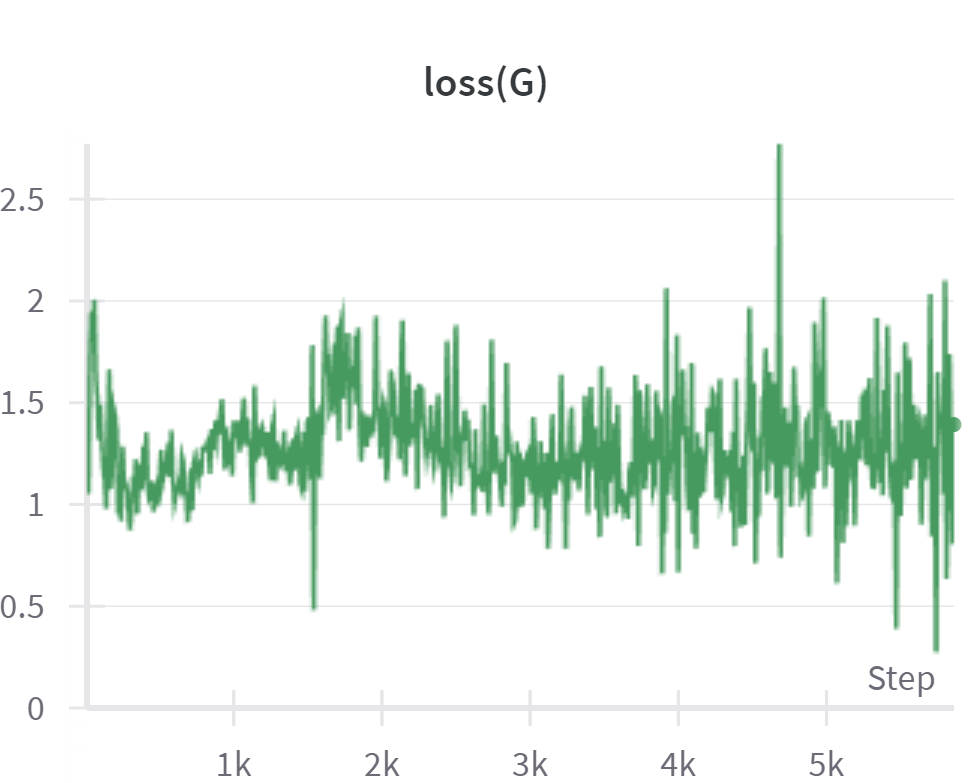
\includegraphics[width=0.95\linewidth]{cifar10/32/lossG.png}
        \caption{}
        \label{subfig:cifar10/32/lossG}
    \end{subfigure}

    \begin{subfigure}{0.45\textwidth}
        \centering
        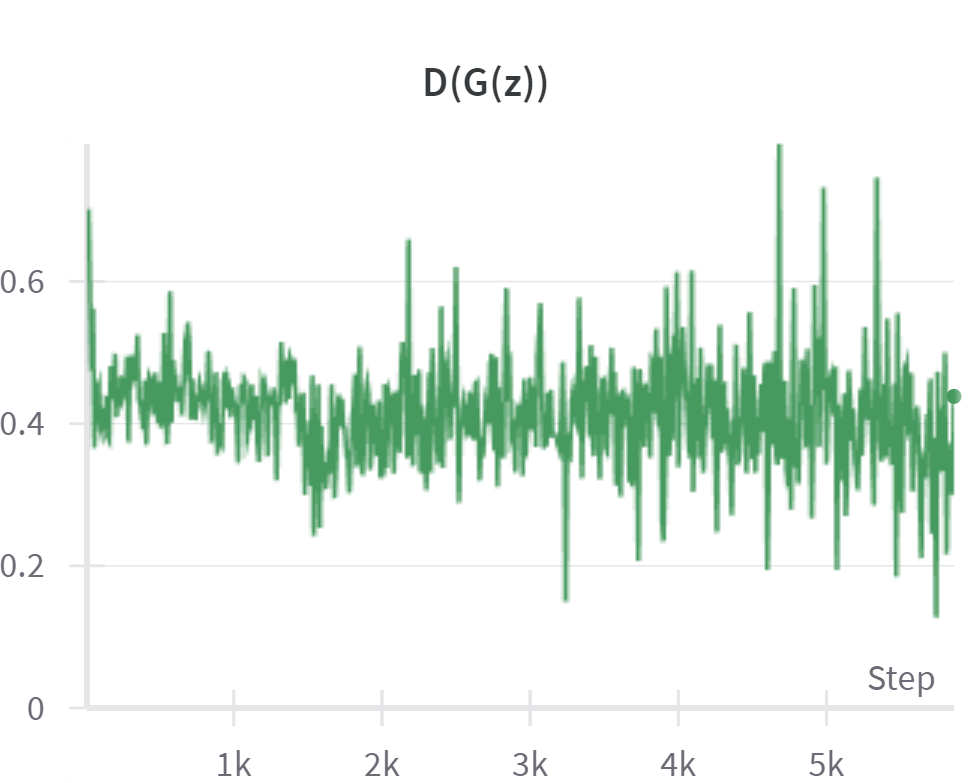
\includegraphics[width=0.95\linewidth]{cifar10/32/D_G_z.png}
        \caption{}
        \label{subfig:cifar10/32/D_G_z}
    \end{subfigure}%
    \begin{subfigure}{0.45\textwidth}
        \centering
        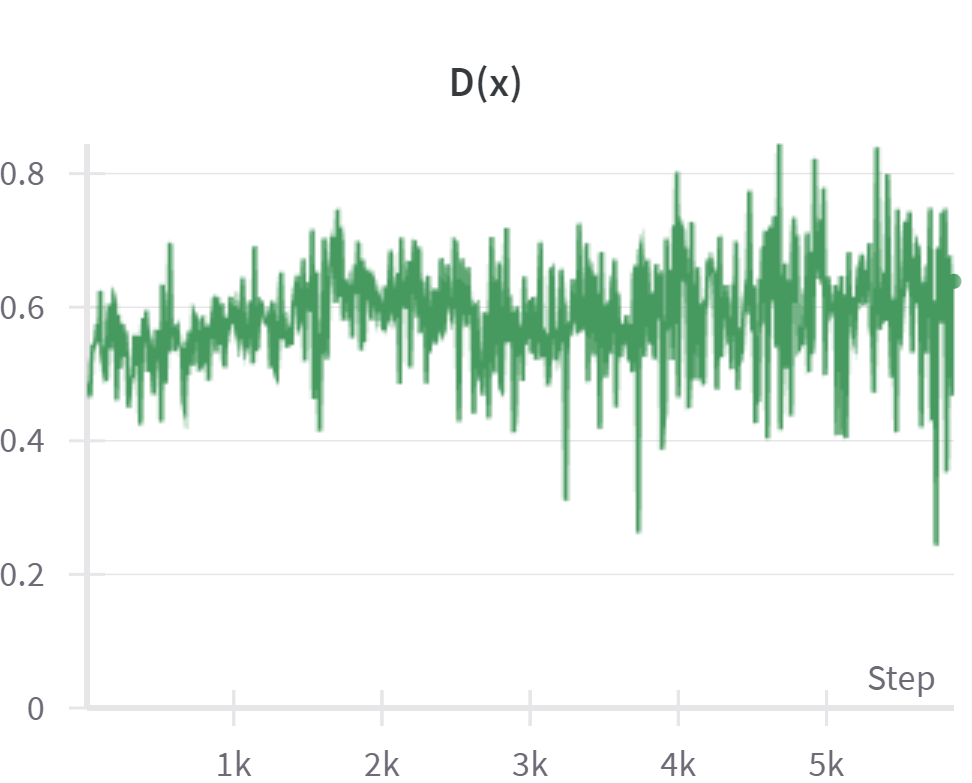
\includegraphics[width=0.95\linewidth]{cifar10/32/D_x.png}
        \caption{}
        \label{subfig:cifar10/32/D_x}
    \end{subfigure}

    \begin{subfigure}{0.45\textwidth}
        \centering
        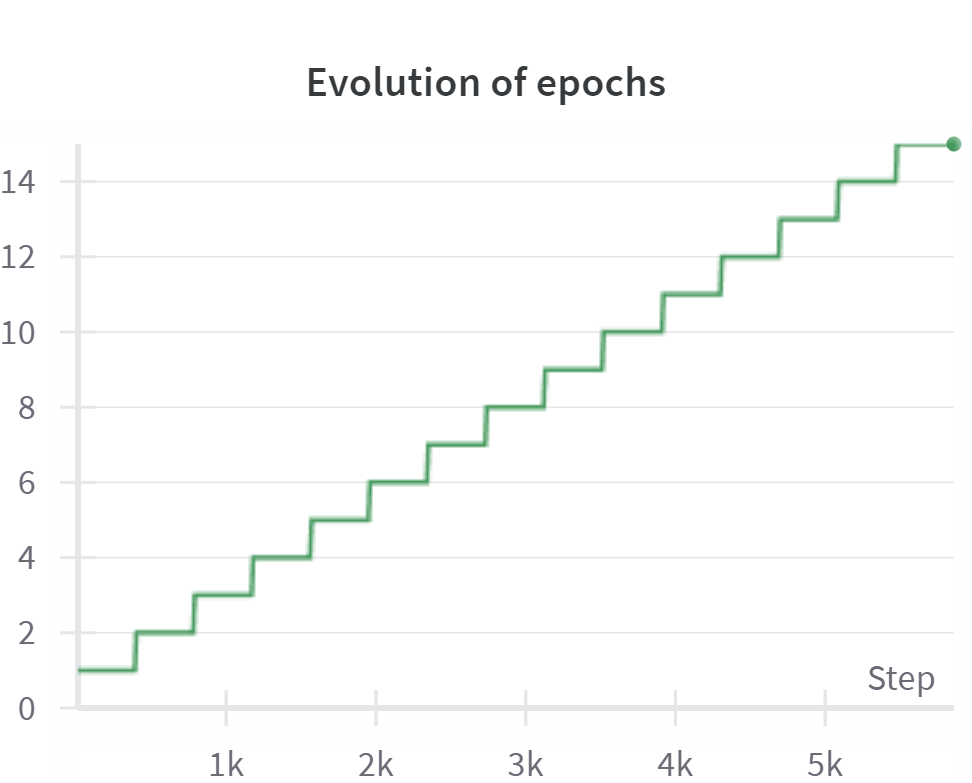
\includegraphics[width=0.95\linewidth]{cifar10/32/epochs.png}
        \caption{}
        \label{subfig:cifar10/32/epochs}
    \end{subfigure}%

    \caption{Training curves: (a) $loss(D)$, (b) $loss(G)$, (c) $D(G(z))$, (d) $D(x)$ and (e) the number of epochs by the number of iterations.}
    \label{fig:cifar10_32_curves}
\end{figure}

\begin{figure}[H]
    \centering

    \begin{subfigure}{0.2\textwidth}
        \centering
        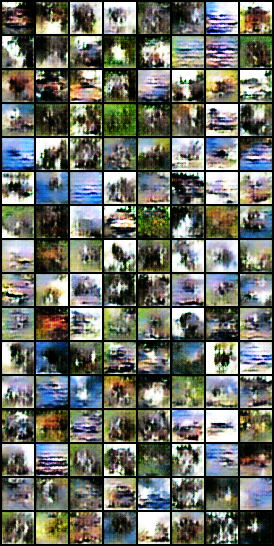
\includegraphics[width=0.95\linewidth]{cifar10/32/fake_sample_epoch_0005.png}
        \caption{}
        \label{subfig:cifar10/32/fake_sample_epoch_0005}
    \end{subfigure}%
    \begin{subfigure}{0.2\textwidth}
        \centering
        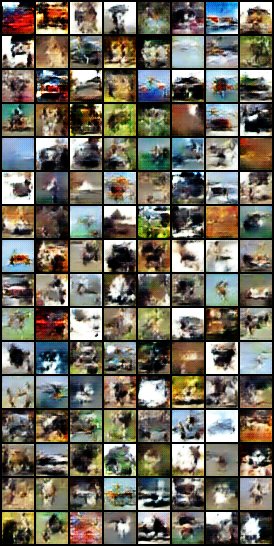
\includegraphics[width=0.95\linewidth]{cifar10/32/fake_sample_epoch_0010.png}
        \caption{}
        \label{subfig:cifar10/32/fake_sample_epoch_0010}
    \end{subfigure}%
    \begin{subfigure}{0.2\textwidth}
        \centering
        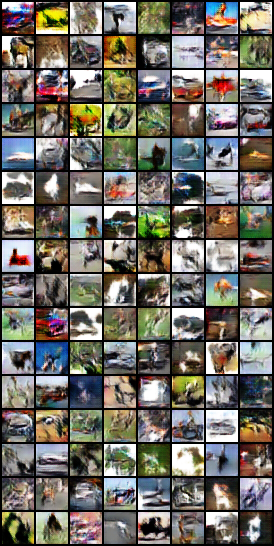
\includegraphics[width=0.95\linewidth]{cifar10/32/fake_sample_epoch_0015.png}
        \caption{}
        \label{subfig:cifar10/32/fake_sample_epoch_0015}
    \end{subfigure}%
    \begin{subfigure}{0.2\textwidth}
        \centering
        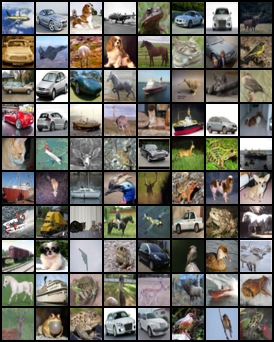
\includegraphics[width=0.95\linewidth]{cifar10/32/real_sample_epoch_0015.png}
        \caption{}
        \label{subfig:cifar10/32/real_sample_epoch_0015}
    \end{subfigure}%

    \caption{Generated $32 \times 32$ CIFAR-10 images using default settings after (a) 5 epochs, (b) 10 epochs and (c) 15 epochs. (d) are examples of real $32 \times 32$ CIFAR-10 images.}
    \label{fig:cifar10_32_images}
\end{figure}

\paragraph*{Generating higher resolution images on CIFAR-10}

To challenge our GAN further and explore its capabilities with higher resolution imagery, we extended our scope from generating $32 \times 32$ CIFAR-10 images to $64 \times 64$ images. This transition necessitated an additional block in our models to accommodate the increased detail and scale, resulting in longer training durations due to the greater complexity of handling larger image sizes.

In this experiment, we observed intriguing results in the training curves, displayed in \Cref{fig:cifar10_64_nz100_curves}. Initially, during the first few epochs, the discriminator was highly proficient at distinguishing between the images generated by the generator, leading to $D(G(z)) \rightarrow 0$. However, as training progressed, G began producing higher-quality images, making it more challenging for D to differentiate between real and fake images. Nevertheless, significant instability is still evident in the training process.

The generated images from this experiment are displayed in \Cref{fig:cifar10_64_images}. To achieve good results, we need much more epochs than in MNIST or when we generated $32 \times 32$ CIFAR-10 images. We can see that at 5 epochs, the images are still blurry, and it's only after 15 epochs that they begin to exhibit some shapes characteristic of the classes in the CIFAR-10 dataset. Even after 30 epochs, they still lack the realism found in the original dataset. However, these shapes are more recognizable than those in the $32 \times 32$ generated images. For instance, the first image located at the top left corner vaguely resembles the red truck from the real images in \Cref{fig:cifar10_64_nz100_real} (third row, second column).

\begin{figure}[H]
    \centering

    \begin{subfigure}{0.2\textwidth}
        \centering
        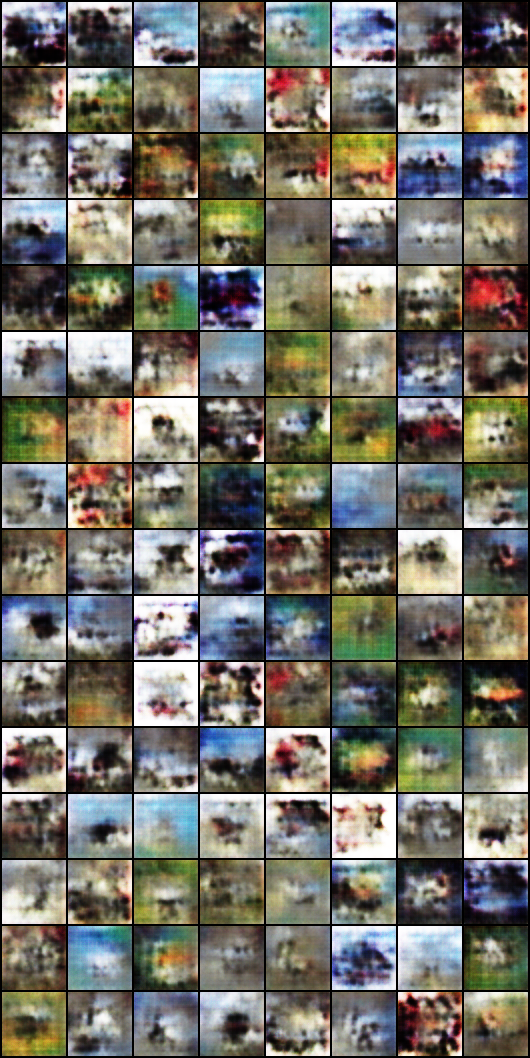
\includegraphics[width=0.95\linewidth]{cifar10/64_nz100/fake_sample_epoch_0005.png}
        \caption{}
        \label{subfig:cifar10/64_nz100/fake_sample_epoch_0005}
    \end{subfigure}%
    \begin{subfigure}{0.2\textwidth}
        \centering
        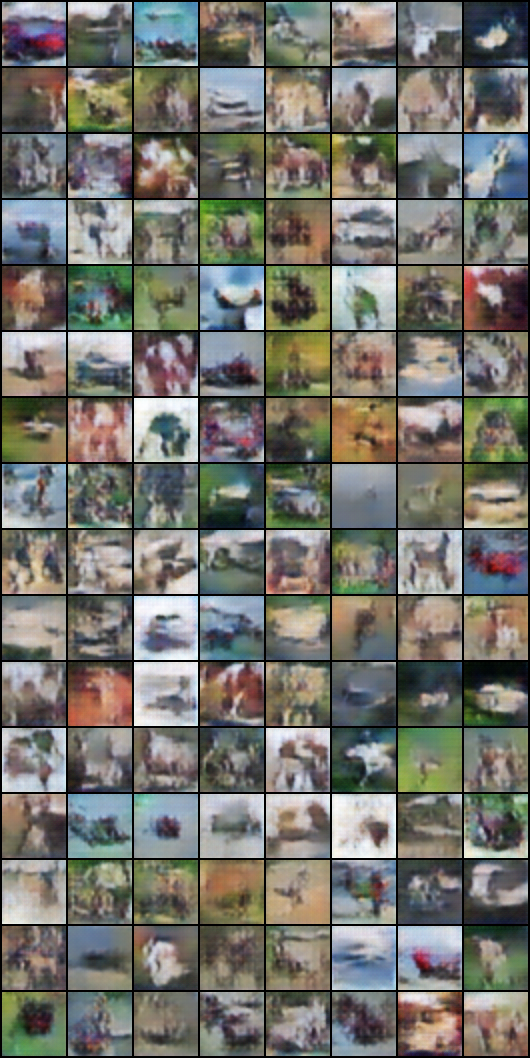
\includegraphics[width=0.95\linewidth]{cifar10/64_nz100/fake_sample_epoch_0010.png}
        \caption{}
        \label{subfig:cifar10/64_nz100/fake_sample_epoch_0010}
    \end{subfigure}%
    \begin{subfigure}{0.2\textwidth}
        \centering
        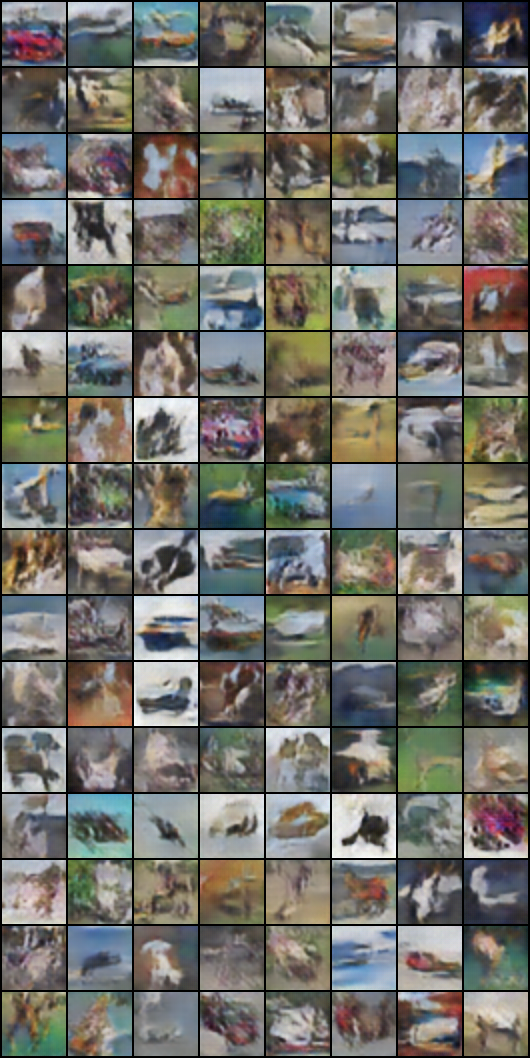
\includegraphics[width=0.95\linewidth]{cifar10/64_nz100/fake_sample_epoch_0015.png}
        \caption{}
        \label{subfig:cifar10/64_nz100/fake_sample_epoch_0015}
    \end{subfigure}%
    \begin{subfigure}{0.2\textwidth}
        \centering
        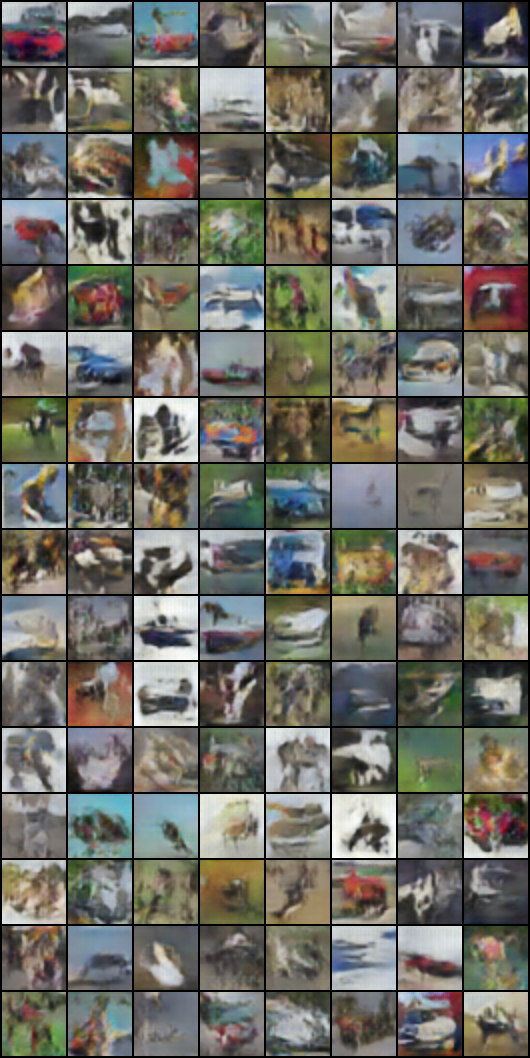
\includegraphics[width=0.95\linewidth]{cifar10/64_nz100/fake_sample_epoch_0020.png}
        \caption{}
        \label{subfig:cifar10/64_nz100/fake_sample_epoch_0020}
    \end{subfigure}%
    % \begin{subfigure}{0.2\textwidth}
    %     \centering
    %     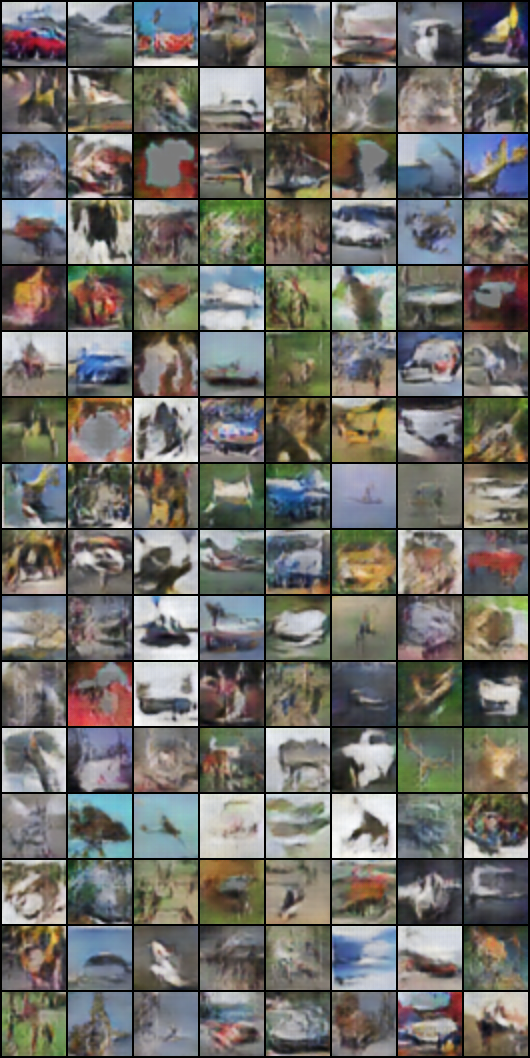
\includegraphics[width=0.95\linewidth]{cifar10/64_nz100/fake_sample_epoch_0025.png}
    %     \caption{}
    %     \label{subfig:cifar10/64_nz100/fake_sample_epoch_0025}
    % \end{subfigure}%
    \begin{subfigure}{0.2\textwidth}
        \centering
        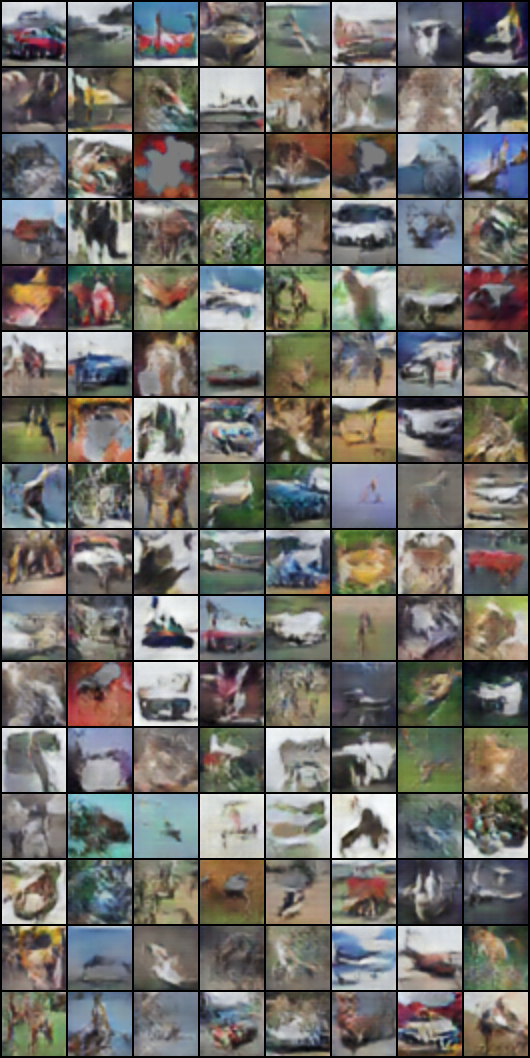
\includegraphics[width=0.95\linewidth]{cifar10/64_nz100/fake_sample_epoch_0030.png}
        \caption{}
        \label{subfig:cifar10/64_nz100/fake_sample_epoch_0030}
    \end{subfigure}

    

    \caption{Generated $64 \times 64$ CIFAR-10 images using default settings after (a) 5 epochs, (b) 10 epochs, (c) 15 epochs, (d) 20 epochs and (e) 30 epochs.}
    \label{fig:cifar10_64_images}
\end{figure}

\begin{figure}[H]
    \centering
    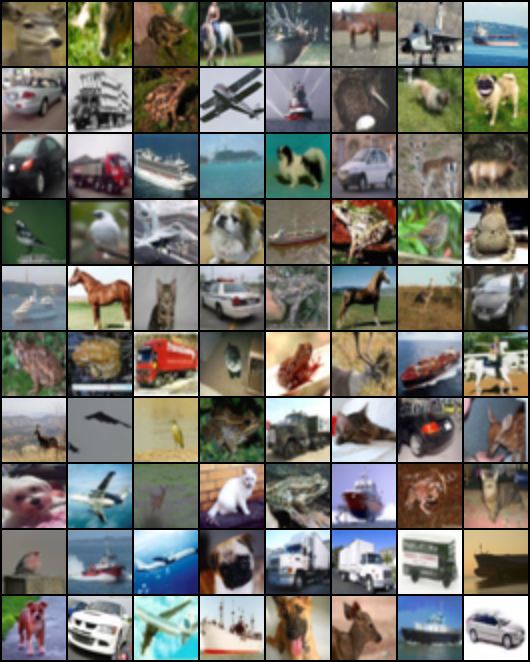
\includegraphics[width=0.2\linewidth]{cifar10/64_nz100/real_sample_epoch_0030.png}
    \caption{Examples of real $64 \times 64$ CIFAR-10 images.}
    \label{fig:cifar10_64_nz100_real}
\end{figure}%

\begin{figure}[H]
    \centering

    \begin{subfigure}{0.45\textwidth}
        \centering
        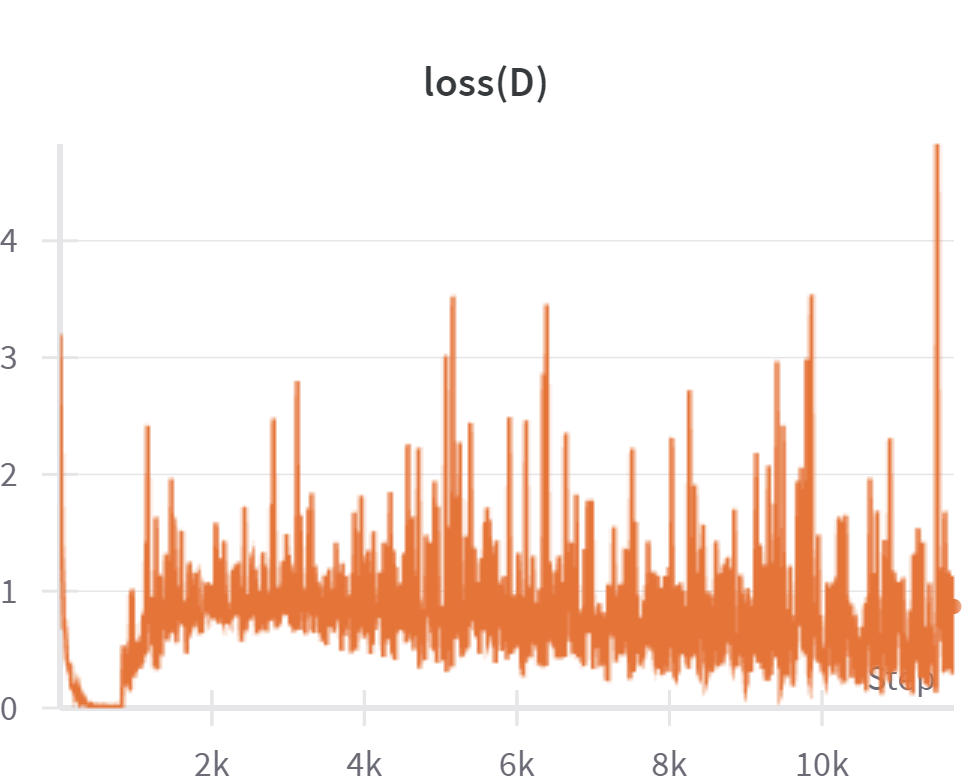
\includegraphics[width=0.95\linewidth]{cifar10/64_nz100/lossD.png}
        \caption{}
        \label{subfig:cifar10/64_nz100/lossD}
    \end{subfigure}%
    \begin{subfigure}{0.45\textwidth}
        \centering
        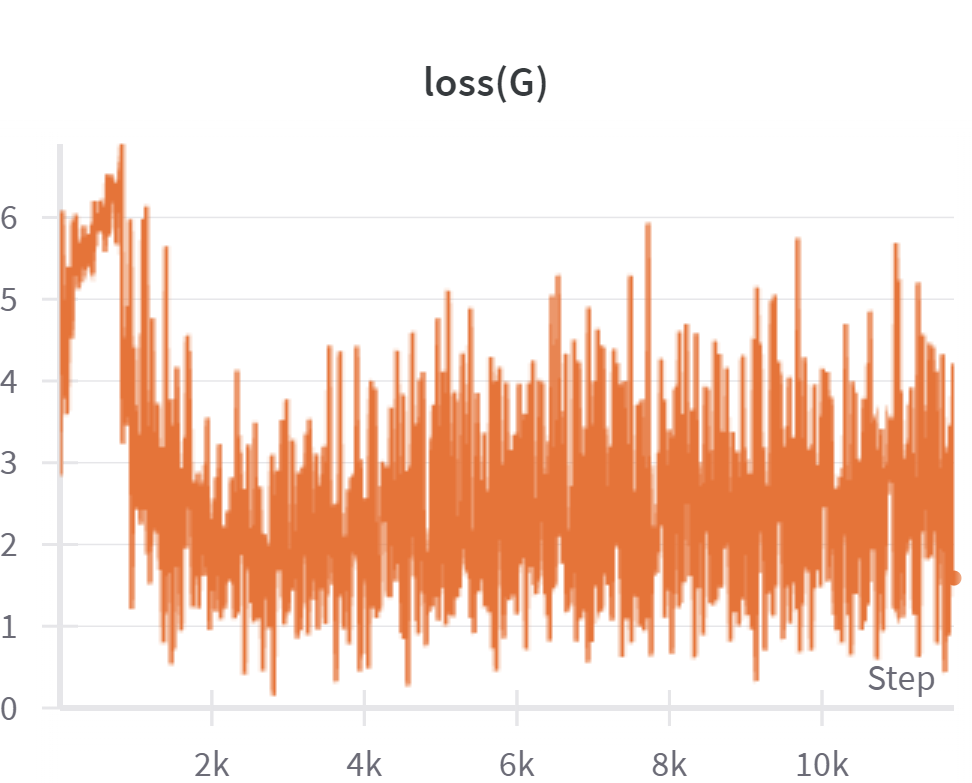
\includegraphics[width=0.95\linewidth]{cifar10/64_nz100/lossG.png}
        \caption{}
        \label{subfig:cifar10/64_nz100/lossG}
    \end{subfigure}

    \begin{subfigure}{0.45\textwidth}
        \centering
        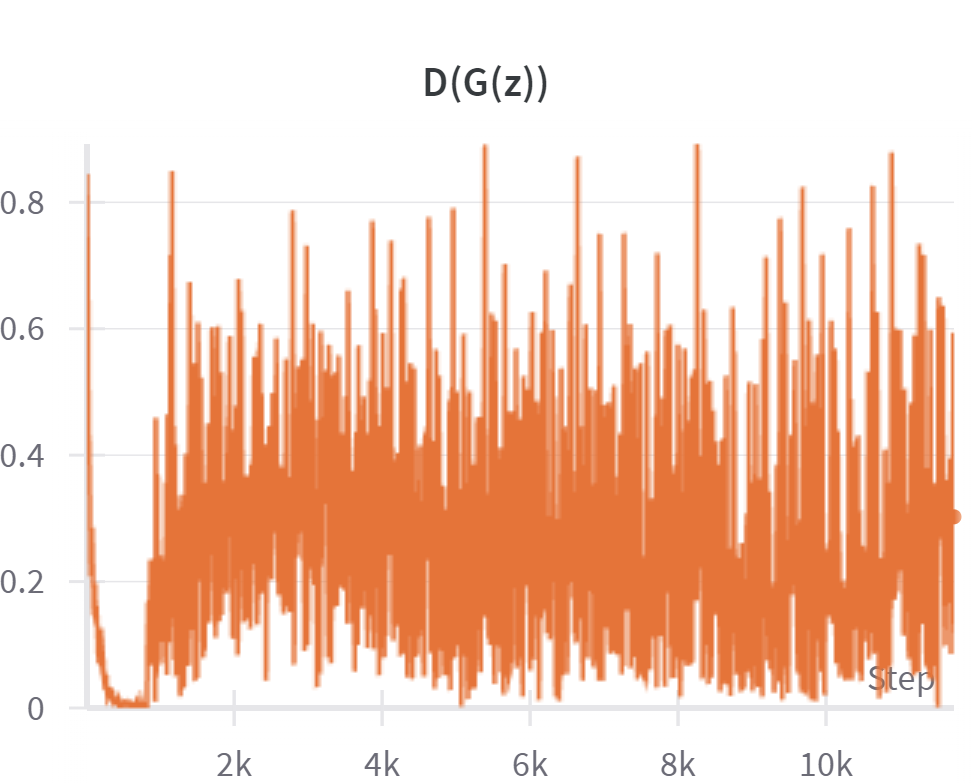
\includegraphics[width=0.95\linewidth]{cifar10/64_nz100/D_G_z.png}
        \caption{}
        \label{subfig:cifar10/64_nz100/D_G_z}
    \end{subfigure}%
    \begin{subfigure}{0.45\textwidth}
        \centering
        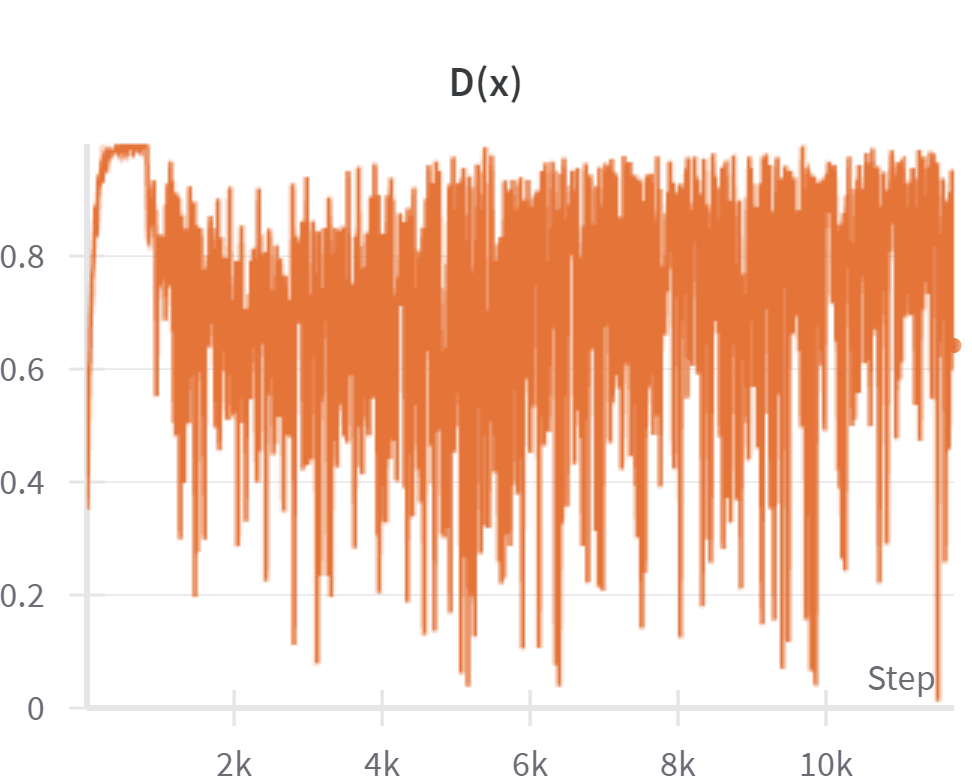
\includegraphics[width=0.95\linewidth]{cifar10/64_nz100/D_x.png}
        \caption{}
        \label{subfig:cifar10/64_nz100/D_x}
    \end{subfigure}

    \begin{subfigure}{0.45\textwidth}
        \centering
        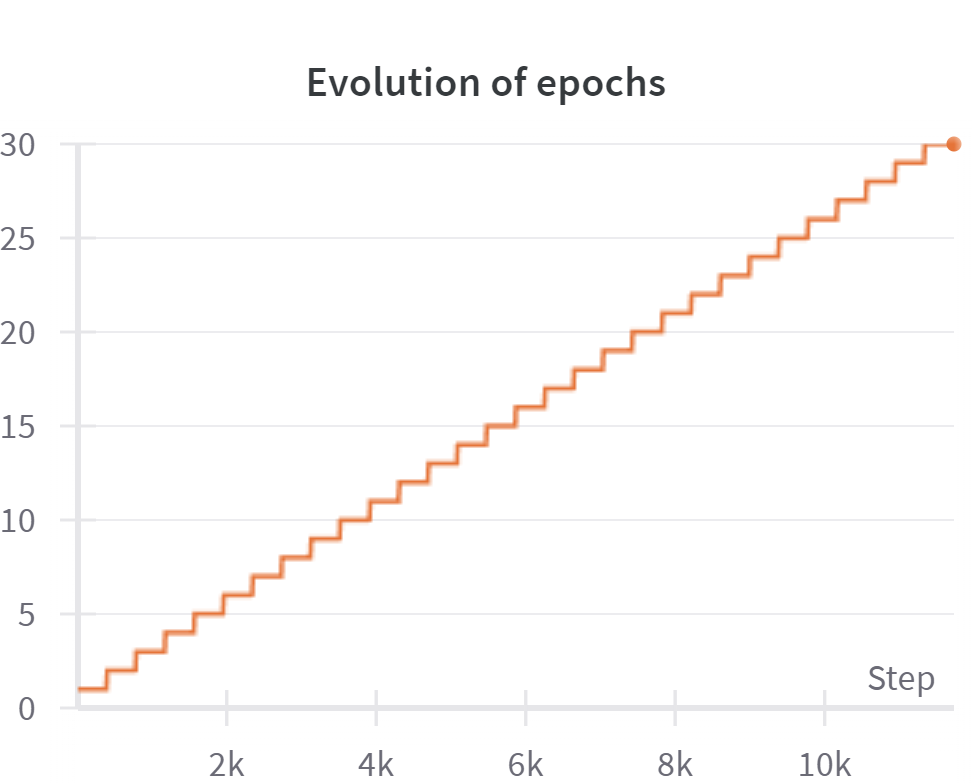
\includegraphics[width=0.95\linewidth]{cifar10/64_nz100/epochs.png}
        \caption{}
        \label{subfig:cifar10/64_nz100/epochs}
    \end{subfigure}%

    \caption{Training curves: (a) $loss(D)$, (b) $loss(G)$, (c) $D(G(z))$, (d) $D(x)$ and (e) the number of epochs by the number of iterations.}
    \label{fig:cifar10_64_nz100_curves}
\end{figure}

Our experiments with GANs reaffirm their complexity in training. Balancing the generator and discriminator, adjusting hyperparameters, and the challenges introduced by conditional variables and image scaling highlight the intricate nature of GANs. Despite these challenges, GANs' ability to generate high-quality images showcases their significant potential, given the right conditions and resources.

\section{Conditional Generative Adversarial Networks}

This section delves into Conditional Generative Adversarial Networks (cGANs), an advanced variant of GANs. We explore how cGANs extend the GAN framework by introducing conditional variables, enabling more control over the generated outputs. We examine how this added layer of control allows for targeted image generation, enhancing the utility of GANs in tasks like image-to-image translation and targeted style transfer. The focus is on understanding the structural differences from standard GANs and the implications of these changes in practical applications.

\subsection{cDCGAN Architectures for MNIST}

\paragraph*{6. Comment on your experiences with the conditional DCGAN.}

Our experience with the conditional DCGAN showed a marked improvement in training stability compared to the unconditional model. Notably, both the generator and discriminator exhibited convergence towards similar values in their respective loss functions within just 5 epochs. This rapid convergence is indicative of a balanced and effective training dynamic. The discriminator maintained slightly more stability than the generator, which is expected as the generator undertook the more complex task of image creation. 

Impressively, the network produced highly recognizable and differentiated images, which underscores the efficacy of conditioning the model, as displayed in \Cref{fig:cDCGAN_default}. This outcome suggests that incorporating conditional variables into the GAN architecture significantly enhances the model's ability to learn and generate targeted, high-quality images rapidly. However, it's worth noting that training takes much longer than a non-conditional GAN, which is a trade-off for the improved stability and control over image generation.

\begin{figure}[H]
    \centering

    \begin{subfigure}{0.2\textwidth}
        \centering
        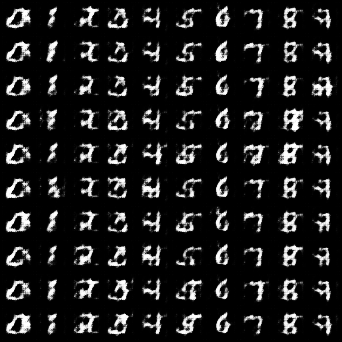
\includegraphics[width=0.95\linewidth]{cDCGAN/fake_sample_epoch_0001.png}
        \caption{}
        \label{subfig:cDCGAN/fake_sample_epoch_0001}
    \end{subfigure}%
    \begin{subfigure}{0.2\textwidth}
        \centering
        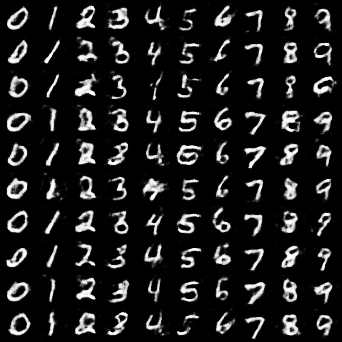
\includegraphics[width=0.95\linewidth]{cDCGAN/fake_sample_epoch_0002.png}
        \caption{}
        \label{subfig:cDCGAN/fake_sample_epoch_0002}
    \end{subfigure}%
    \begin{subfigure}{0.2\textwidth}
        \centering
        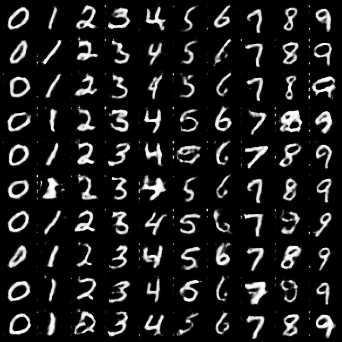
\includegraphics[width=0.95\linewidth]{cDCGAN/fake_sample_epoch_0003.png}
        \caption{}
        \label{subfig:cDCGAN/fake_sample_epoch_0003}
    \end{subfigure}%
    \begin{subfigure}{0.2\textwidth}
        \centering
        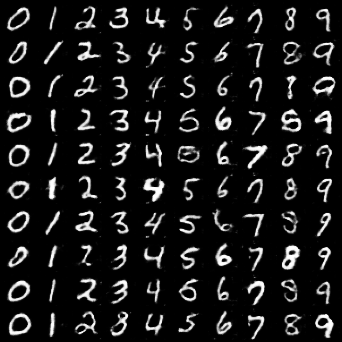
\includegraphics[width=0.95\linewidth]{cDCGAN/fake_sample_epoch_0004.png}
        \caption{}
        \label{subfig:cDCGAN/fake_sample_epoch_0004}
    \end{subfigure}%
    \begin{subfigure}{0.2\textwidth}
        \centering
        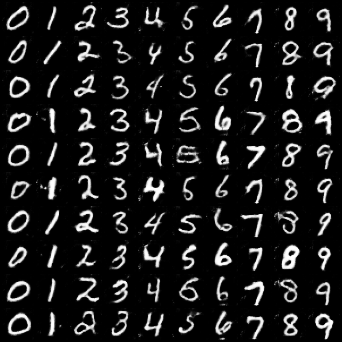
\includegraphics[width=0.95\linewidth]{cDCGAN/fake_sample_epoch_0005.png}
        \caption{}
        \label{subfig:cDCGAN/fake_sample_epoch_0005}
    \end{subfigure}

    

    \caption{Generated digits from a cDCGAN during training using default settings after (a) 1 epoch, (b) 2 epochs, (c) 3 epochs, (d) 4 epochs and (e) 5 epochs.}
    \label{fig:cDCGAN_default}
\end{figure}

% ça marche bien ?

\paragraph*{7. Could we remove the vector $y$ from the input of the discriminator (so having $cD(x)$ instead of $cD(x, y)$)?}

Removing the vector $y$ from the input of the discriminator in a conditional cGAN would significantly alter the network's nature and functionality. The discriminator's role would be reduced to assessing the realism of the images, without the capability to evaluate whether the generated images meet the specified conditions. Consequently, it would be unable to determine whether a generated digit image corresponds to the provided digit label. On the other hand, the generator would still receive $y$ as input. However, with the discriminator no longer enforcing condition compliance, there would be less motivation for the generator to produce images that conform to the specific conditions. This would lead the network towards generating generic, realistic images that may not necessarily align with the intended conditional attributes.

In our experiment, we modified the code to employ an unconditional discriminator while keeping a conditional generator. Our observations supported our hypotheses: because the discriminator lacks conditioning, the generator is not compelled to align with specific conditional inputs. Consequently, the latent space is not effectively conditioned, leading to a lack of consistent correspondence between specific conditions and the generated images. This was evident as the digits appeared to 'move' positions during training, as the discriminator did not impose any particular condition.

The resulting images in \Cref{fig:cgan_mnist}, although generated, did not conform to the conditional constraints we had defined.  Additionally, we observed mode collapse, where each digit is only associated once, meaning that certain digits were not being adequately represented in the generated samples, leading to a lack of diversity in the output. This underscores the critical role of a conditional discriminator in a cGAN framework, as it ensures that the generated images align with the specified conditions and helps prevent mode collapse by encouraging diversity in the generated samples.

\begin{figure}[H]
    \centering
    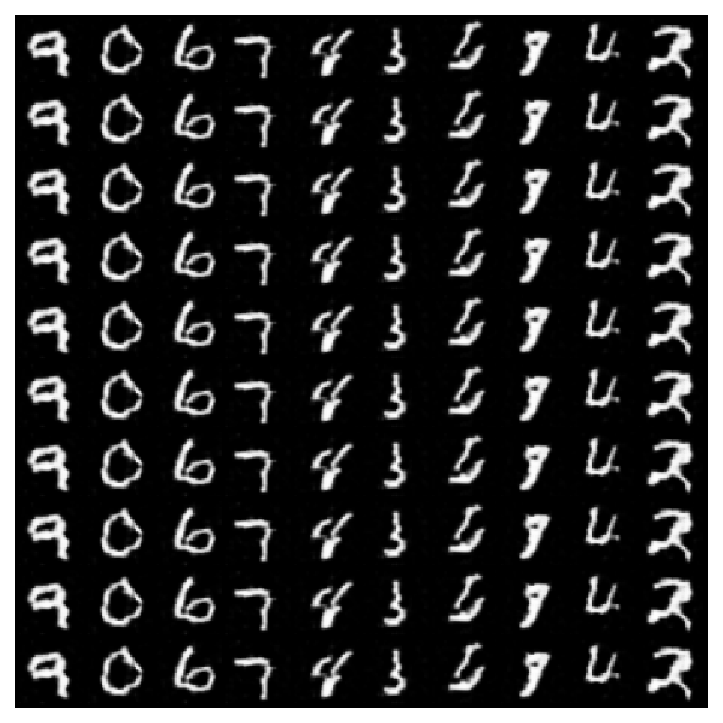
\includegraphics[width=.5\textwidth]{cgan_mnist}
    \caption{Generated digits from a cDCGAN trained for 10 epochs with the removal of the vector $y$ from the input of the discriminator.}
    \label{fig:cgan_mnist}
\end{figure}

\paragraph*{8. Was your training more or less successful than the unconditional case? Why?}

The training in the conditional case can be considered more successful compared to the unconditional one primarily because the introduction of the conditioning variable $ y $ allows the GAN to generate images that are conditioned on specific attributes or classes. This directed generation process can lead to a more controlled and diverse output. For example, in an unconditional GAN, without $ y $, the generator has no guidance on what type of image to produce, which can sometimes result in mode collapse, where the generator produces very similar or even the same images repeatedly.

However, with the conditional GAN, each $ y $ corresponds to a different attribute or class label. This means that for each different $ y $, the generator is tasked with producing an image that not only looks realistic but also matches the given condition. This helps to ensure that the generator produces a diverse set of images across different classes or attributes, effectively avoiding mode collapse. The discriminator, in turn, has to learn to judge not just the realism, but also the correctness of the conditioned output. This makes the training more robust and the model more versatile, as it learns a richer representation of the data.

\paragraph*{9. Test the code at the end. Each column corresponds to a unique noise vector $z$. What could $z$ be interpreted as here?}

In this context, the noise vector $z$ can be interpreted as the source of randomness or variability that the generator $G$ utilizes to produce different outputs. Each column in \Cref{fig:impact_of_z} corresponds to a unique $z$, and since $z$ is repeated for each class, it serves as a means to generate variations of images across different classes.

Essentially, $z$ acts as a seed for the generative process. Different seeds are expected to yield different images, and with the repetition of $z$ across classes, it's used to generate diverse variations of images corresponding to each class label provided in $y_s$. In summary, $z$ introduces the stochastic element that, in conjunction with class labels, enables the generator to create a variety of images within the specified classes.

\begin{figure}[H]
    \centering
    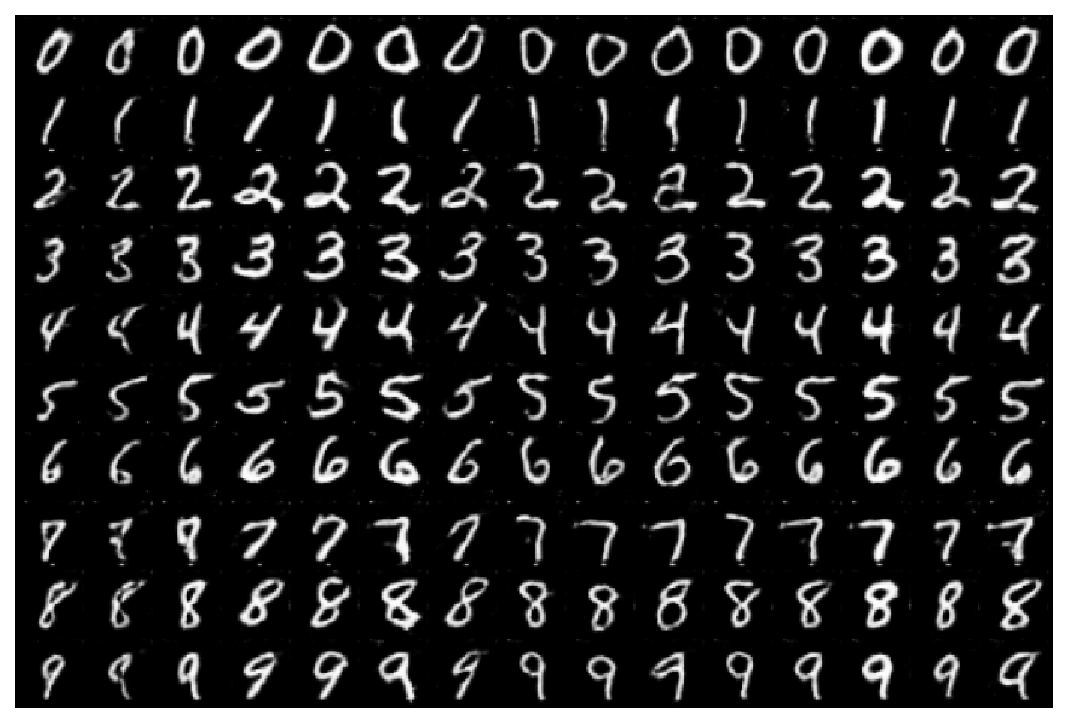
\includegraphics[width=.8\textwidth]{impact_of_z}
    \caption{Influence of a unique noise vector $z$ on our cGAN's generated images.}
    \label{fig:impact_of_z}
\end{figure}